\documentclass[11pt,a4paper]{report}
\usepackage[utf8]{inputenc}
\usepackage{amsmath}
\usepackage{amsfonts}
\usepackage{amssymb}
\usepackage{graphicx}
\usepackage[left=3cm,right=3cm,top=3cm,bottom=3cm]{geometry}
\author{\textbf{Por: Alejandro Tirado, Renzo Cocha, Andres Saltos, Alejandra Flores}}
\title{\textbf{MENSAJERIA INSTANTANEA}}
\date{}
\begin{document}
\maketitle
\begin{center}
\large \textbf{INTRODUCCION}
\end{center}
Se va a informar sobre el desarrollo del proyecto, poner en manifiesto y mostrar los\vspace{0,5cm} resultados, así como la conclusión para la realización del proyecto denominado\vspace{0,5cm} “MENSAJERÍA INSTANTÁNEA PARA COMPUTADORA” el cual se desarrollara mediante la realización\vspace{0,5cm} de un prototipo baja fidelidad.
Se mostrara el avance realizado en el cual\vspace{0,5cm} se pudo definir las características principales que tendrá la aplicación también como el\vspace{0,5cm} diseño, el cual se define que contara con las opciones principales y necesarias que requiere\vspace{0,5cm} una mensajería instantánea.
Puesto que la finalidad del informe es dar a conocer las\vspace{0,5cm} primeras ideas del proyecto a realizar y así visualizar lo que vamos a implementar en dicha\vspace{0,5cm} aplicación, la cual se va a realizar bajo el lenguaje de programación Java que es el más\vspace{0,5cm} conveniente referente a los conocimientos adquiridos a lo largo de la carrera hasta ahora.\newpage

\textbf{OBJETIVOS}\newline\\

\textbf{Objetivo general}\vspace{0,5cm}

• Mostrar los avances que se han realizado en el proyecto de la realización de mensajería instantánea. \vspace{0,5cm}

\textbf{Objetivo Especificos}\newline\\


•	Detallar  las nuevas funciones y características que se ha realizado en la aplicación.\newline\\

•	Mostrar los avances que hemos tenido en el programa. \newline\\

•	Definir las nuevas propuestas para mejorar las nuevas funciones realizadas.\newpage
 

\textbf{DESARROLLO}\vspace{0,5cm}

Para realizar el prototipo de baja fidelidad para el software de mensajería instantánea\vspace{0,5cm}  que se utilizara en computadora, primeramente se optó por diseñar la interfaz mediante\vspace{0,5cm} un esquema realizado a mano.\vspace{0,5cm}


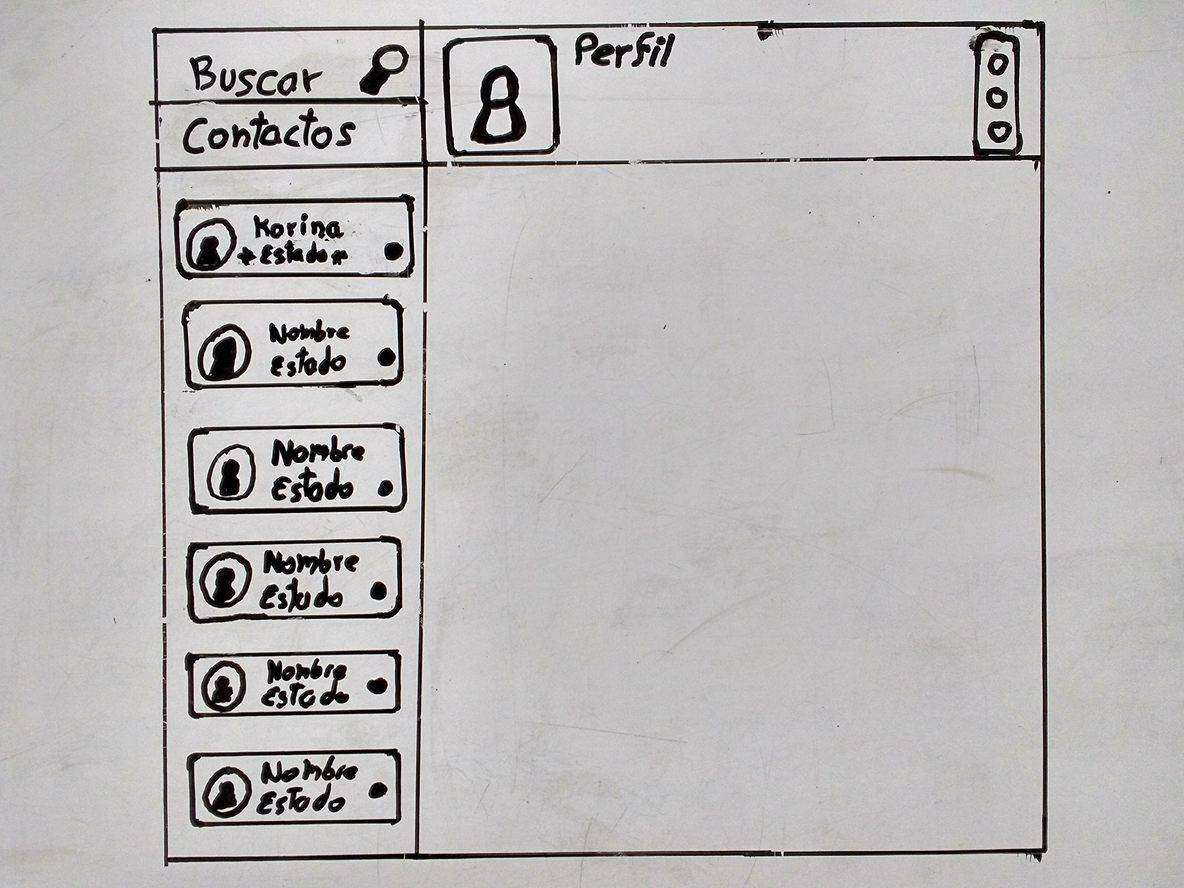
\includegraphics[scale=0.1]{../../instantmessenger/prbd2.jpg} 
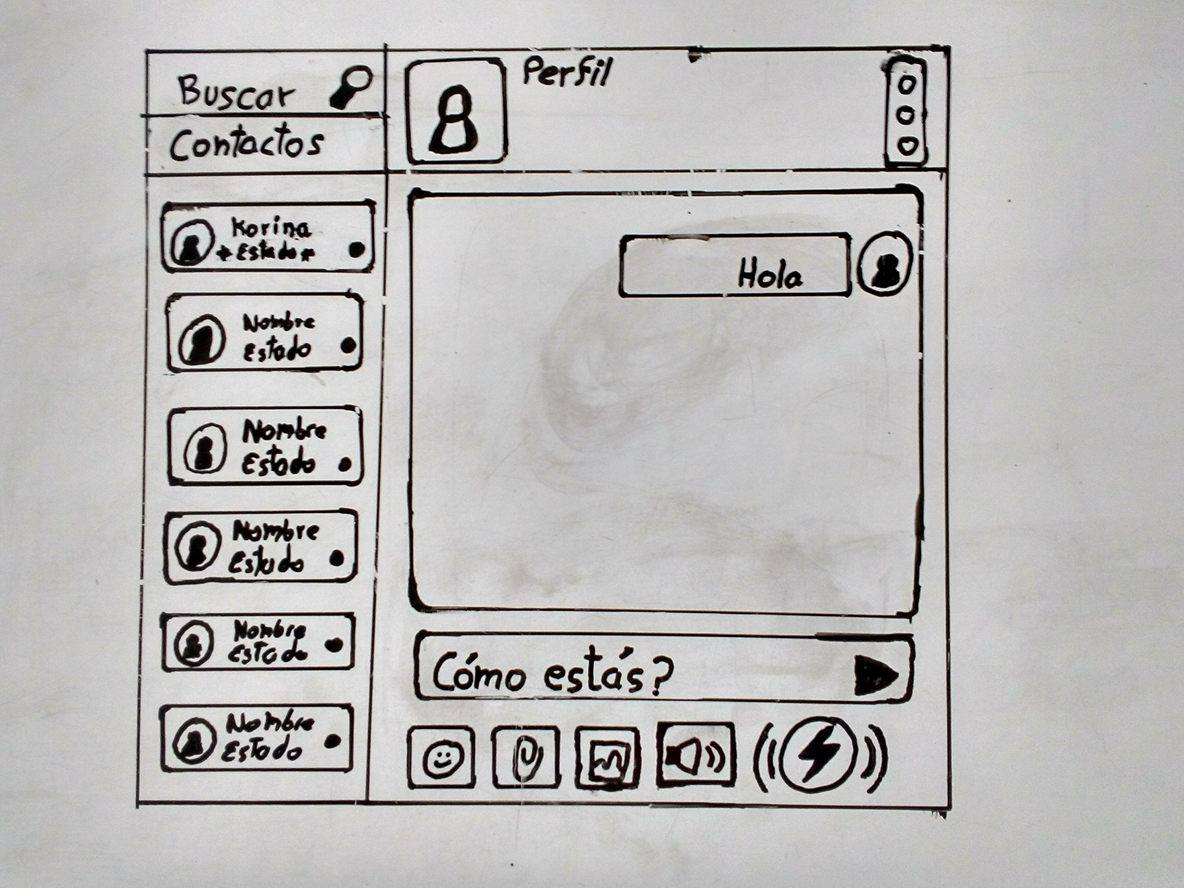
\includegraphics[scale=0.1]{../../instantmessenger/prbd1.jpg} 
 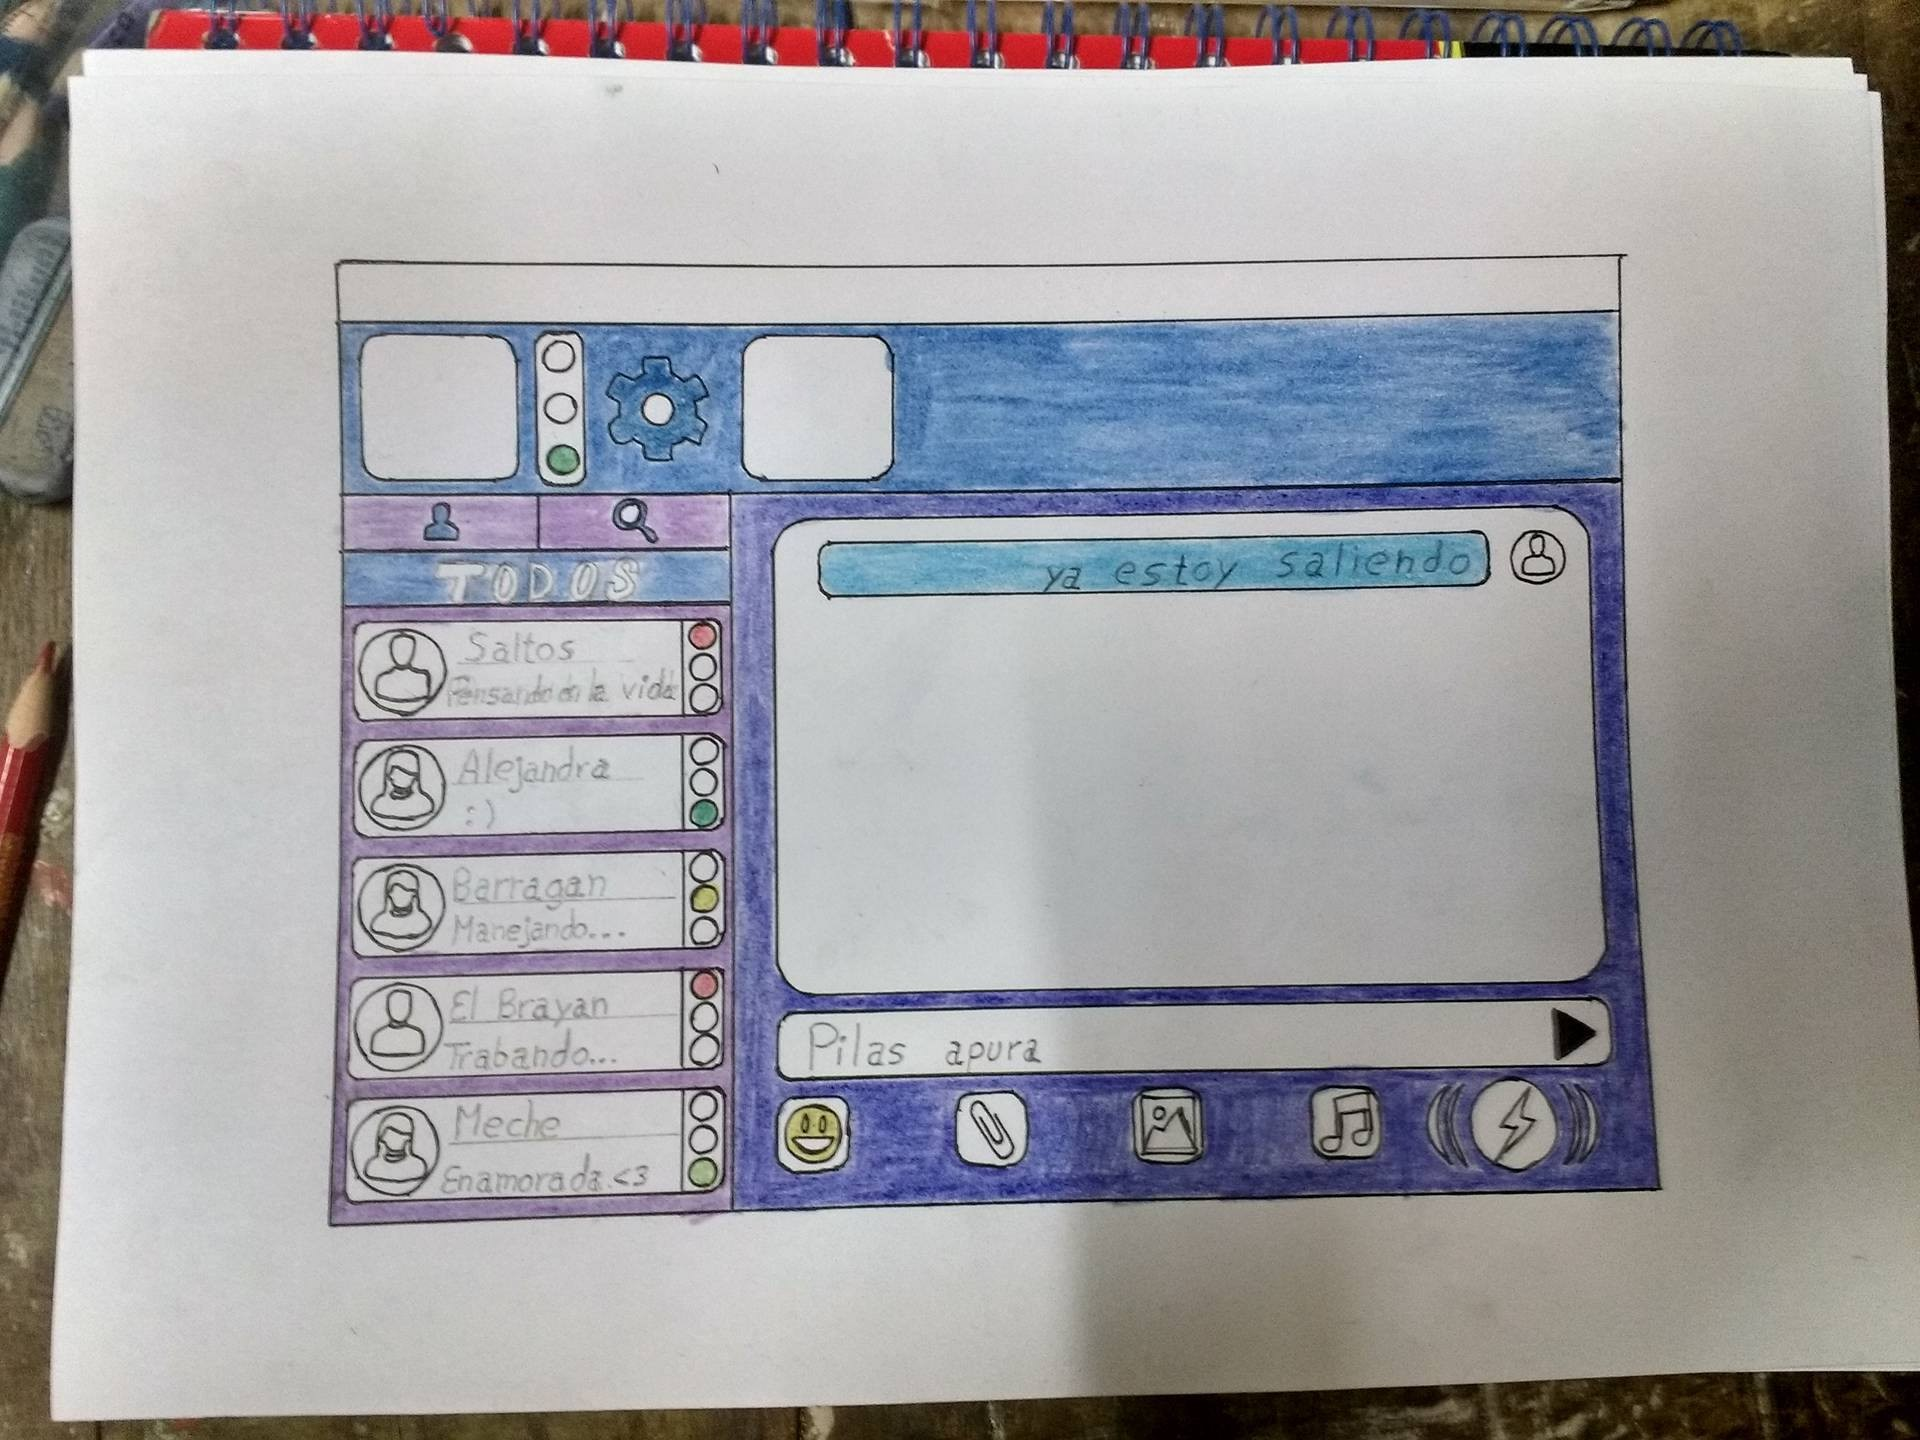
\includegraphics[scale=0.1]{../../instantmessenger/prbd3.jpg} \newpage

Mediante el desarrollo del esquema se pudo definir las características principales que\vspace{0,5cm} tendrán el software de mensajería instantánea así como también el logotipo, diseño  y su\vspace{0,5cm} nombre el cual se llamara 3ArChat. 
3ArChat  será una aplicación para computadoras que\vspace{0,5cm} permitirá interactuar mediante mensajes instantáneos, sus características son:\newline\\ 
Nombre.\newline\\
Estado.\newline\\ 
Envió de música.\newline\\ 
Envió de zumbidos.\newline\\
Envió de archivos pdf.\newline\\ 
Envió de imágenes.\newline\\ 
Visualizar imagen, videos ,sonidos, PDF.\newline\\ 
Búsqueda de contactos.\newline\\
Agregar contacto.\newline\\ 
Bloquear contacto.\newline\\ 
Editar estado y foto de perfil.\newline\\
Cambiar color del chat.\newline\\ 
Fondo  de chat.\newline\\ 
Eliminar conversación.\newline\\ 
También\vspace{0,5cm} podemos observar que en la ventana de chats están nuestros contactos con su estado y foto\vspace{0,5cm} de perfil. En la parte inferior la barra de opciones para poder seleccionar lo que queramos\vspace{0,5cm} utilizar junto a la opción de enviar emojis.
En la parte superior de la venta nuestra\vspace{0,5cm} información como foto y la del usuario con el que estaremos enviando mensajes instantáneos,\vspace{0,5cm} así mismo la opción de ajustes para poder editar nuestra información personal.\newpage

\textbf{NUEVAS FUNCIONES}\vspace{0,5cm}
\begin{itemize}
\item Registro para otros usuarios. 
\item Validación de usuario
\item Visibilidad de contraseña
\item Opción de recuperación de contraseña
\item Probar otros tipos de letra
\item Tamaño de letra
\item Colores para pantalla principal del chat.

\end{itemize}\newpage




\textbf{CONCLUSIONES}\newline\\ 

•	Mediante el análisis que pudimos tener se pudo realizar el prototipo de baja fidelidad para el software de mensajería instantánea que iremos realizando  conforme obtengamos los conocimientos necesarios para este proyecto\newline\\ 

•	Diseñamos el esquema de la interfaz que tendrá la aplicación de mensajería que nos permite tener una idea visual de cómo se verá más adelante dicha aplicación.\newline\\ 


•	Detallamos  las funciones y características que tendrá la aplicación las cuales son óptimas y necesarias  para las necesidades del usuario  ya que esta aplicación nos va a permitir enviar archivos pdf, música e imágenes.\newline\\ 


•	Definimos que el software que se va a utilizar para el desarrollo de la aplicación será el lenguaje de programación Java.\newpage

\textbf{COMENTARIOS} \newline\\

¿Qué te parece la interfaz del chat y que te gustaría agregarle?\newline\\

• Excelente se ve muy dinámica.\newline\\

• Me encanta la idea de los semáforos!\newline\\

• No me gusta mucho lo de los semáforos preferiría que solo aparezca un botón no los\vspace{0,5cm} tres al mismo tiempo. 
Pues me gusta mucho la idea del zumbido como lo era en Messenger.\newline\\

• Esta aceptable.




\end{document}